
\section{Реализация математической модели}\label{sec:ch2/sec5}

Обобщая полученные ранее результаты математического моделирования,
представим полную систему уравнений, описывающую динамику электропневматического
привода с дискретными распределителями:

\begin{equation}\label{eq:ch2/final_system_raw}
    a=1.
    % \begin{cases}
    %     \begin{alignedat}[2]
    %     \end{alignedat}
    % \end{cases}    
\end{equation}

Для повышения эффективности численной реализации данная система была
оптимизирована путем применения векторизации уравнений, оптимизации нелинейных
функций и аналитического вычисления якобиана, которое описано в Приложении \ref{app:A}.
Эти оптимизации позволили существенно повысить производительность вычислений при проведении многочисленных
итераций в задачах анализа и синтеза алгоритмов управления.

В результате получена следующая векторизованная форма системы:

\begin{equation}\label{eq:ch2/final_system}
    \begin{cases}
        \begin{alignedat}{2}
            \dot{x}               & = v                                                                                                                                                                                                   \\
            M\dot{v}              & = \mathbf{F}^T\mathbf{p} - p_\text{атм}(\mathbf{F}^T\mathbf{1}) - R_\text{тр}(v) - R_\text{оп}(x, v)                                                                                                  \\
            \dot{\mathbf{p}}      & = \frac{\gamma}{\mathbf{V}(\mathbf{x})} \odot (R\mathbf{T} \odot \mathbf{G} - \mathbf{p} \odot (\mathbf{F}v))                                                                                         \\
            \dot{\mathbf{T}}      & = \frac{\gamma-1}{\mathbf{m}C_v} \odot (R\mathbf{T} \odot \mathbf{G} \pm \mathbf{p} \odot (\mathbf{F}v))                                                                                              \\
            \mathbf{u}_\text{зад} & = \tau \dot{\mathbf{u}} + \mathbf{u}                                                                                                                                                                  \\
            \mathbf{G}            & = \psi(\mathbf{p}_\text{вх}, \mathbf{p}_\text{вых}) \odot \mathbf{C}_d \odot \mathbf{F}_\text{пр} \odot \mathbf{u} \odot \frac{\mathbf{p}_\text{вх}}{\sqrt{R\mathbf{T}_\text{вх}}}                    \\
            R_\text{тр} &= \sigma_0 z + \sigma_1 \dot{z} + \sigma_2 v                                                                                                                              \\
            \dot{z} &= v - \frac{\sigma_0 |v|}{g(v)}z \\
            R_\text{оп}           & = k_\text{оп}(x - x_\text{мин})\cdot \frac{1}{1 + e^{-\alpha(x - x_\text{мин})}} + k_\text{оп}(x - x_\text{макс})\cdot \frac{1}{1 + e^{-\alpha(x - x_\text{макс})}}                                   \\
        \end{alignedat}
    \end{cases}
\end{equation}

На основе оптимизированной математической модели разработана функциональная блок-схема,
представленная на рисунке \ref{fig:ch2/block_diagram}, которая отражает
взаимосвязи между различными компонентами модели и порядок вычислений.

\begin{figure}[ht]
    \centerfloat{
        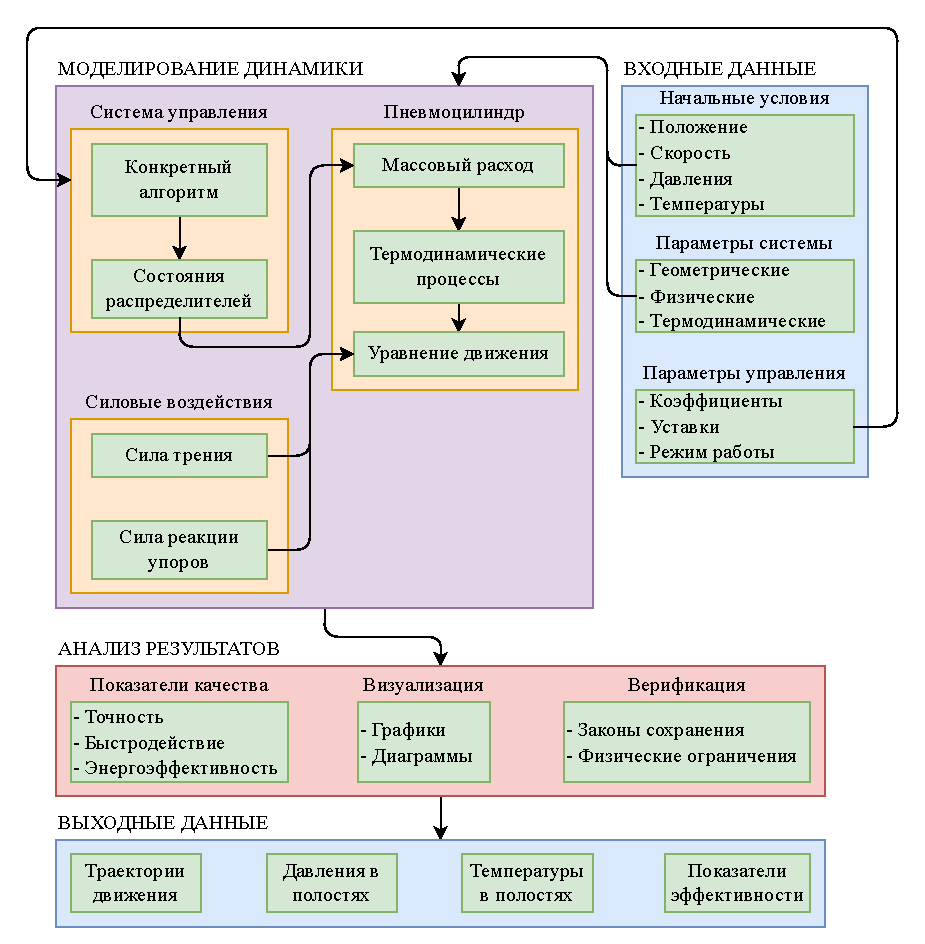
\includegraphics[]{part2/diagrams/pneumatic_actuator_functional_block_diagram.pdf}
    }
    \caption{Функциональная блок-схема математической модели электропневматического привода}
    \label{fig:ch2/block_diagram}
\end{figure}

Программная реализация математической модели выполнена на языке Python с применением объектно-ориентированного подхода.
Архитектура программного комплекса построена на принципах модульности и инкапсуляции, что обеспечивает гибкость при модификации отдельных компонентов системы.

Центральным элементом реализации является класс \texttt{PneumaticCylinder}, инкапсулирующий
математическую модель пневматического привода в векторизованной форме. Структура класса включает:
\begin{itemize}
\item Систему дифференциальных уравнений в векторной форме;
\item Модели нелинейных эффектов через отдельные классы \texttt{FrictionModel} и \texttt{StopForce};
\item Термодинамические процессы в рабочих полостях;
\item Динамику переключения распределителей.
\end{itemize}

Численное интегрирование системы осуществляется методом BDF (Backward Differentiation Formula),
оптимальным для решения жёстких систем дифференциальных уравнений. Эффективность интегрирования
значительно повышена за счет применения аналитически вычисленного якобиана (см. Приложение \ref{app:A3}), что позволило существенно сократить вычислительные затраты.

Визуализация результатов моделирования реализована с применением библиотеки Matplotlib,
обеспечивающей построение графиков временных зависимостей основных параметров системы: перемещения
и скорости поршня, давлений и температур в полостях цилиндра, состояний распределителей. Программный
комплекс предусматривает возможность экспорта результатов в различные форматы для последующей обработки и анализа.

Разработанная программная реализация обеспечивает возможность эффективного проведения
вычислительных экспериментов, параметрической оптимизации и анализа динамических характеристик
пневматического привода. Модульная структура программного комплекса позволяет легко модифицировать
отдельные компоненты системы и интегрировать новые алгоритмы управления.